\chapter{Reti di Petri}
\section{Introduzione}
Le reti di Petri sono un modello formale per la descrizione di sistemi
distribuiti a tempo discreto \footnote{Le reti di Petri possono essere
generalizzate, in modo da trattare anche sistemi distribuiti a tempo
continuo.}. A differenza delle algebre di processo, come il CCS,
le reti di Petri permettono di descrivere la true concurrency di un
sistema concorrente, usando una semantica a ordine parziale.
Le algebre di processo, infatti, descrivono l'evoluzione (sequenziale) dello
stato globale del sistema. Molto spesso, però, lo stato globale del sistema
concorrente non è conosciuto, e risulta più rilevante trattare gli stati
locali e la loro evoluzione: le reti di Petri, quindi, permettono di
rappresentare gli stati locali, senza dover essere necessariamente
a conoscenza dello stato globale.

Le reti di Petri, oltre che rappresentare formalmente sistemi concorrenti,
permettono anche di verificarne alcune proprietà.
In particolare, come si vedrà, proprietà importanti come la raggiungibilità o
presenza di deadlock possono essere verificate usando il grafo dei casi,
mentre proprietà più complesse possono essere verificate tramite il model
checking con formule HTL.
Alcuni problemi di decisione su reti di Petri sono stati studiati da
Esparza e Nielsen (1995) METTERE CITAZIONE.

\section{Reti elementari e grafi dei casi}
Il tipo di rete di Petri più basilare è una rete elementare, detta anche
sistema elementare.
In questo tipo di rete, tutti gli stati hanno una capacità massima di un token,
gli archi hanno peso 1 e non sono presenti token colorati, ovvero tutti i
token rappresentano lo stesso tipo di dato.

\begin{defn}
    Una \textbf{rete} è una tripla $(P, T, F)$, dove:
    \begin{itemize}
        \item $P$ è l'insieme finito dei posti che compongono la rete.
        \item $T$ è l'insieme finito delle transizioni che compongono la rete.
        \item $F \subseteq (P \cup T) \times (T \times P)$ è la relazione
        di flusso, che stabilisce quali posti e transizioni sono collegati
        da archi diretti
        \footnote{Si può osservare che una rete definisce un grafo bipartito,
        dove i due sottoinsiemi che definiscono la partizione sono $P$ ed $T$.}.
        La relazione di flusso non può collegare tra loro posti o transizioni.
    \end{itemize}
\end{defn}

\begin{rem}
    Le reti vengono solitamente assunte T-ristrette, ovvero ogni transizione
    deve avere almeno una precondizione (e quindi un arco entrante) e
    almeno una postcondizione (e quindi un arco uscente).
\end{rem}

\begin{defn}
    Siano $N_1 = (P_1, T_1, F_1)$ e $N_2 = (P_2, T_2, F_2)$ due reti,
    $N_2$ è \textbf{sottorete} di $N_1$ sse:
    \begin{itemize}
        \item $P_2 \subseteq P_1$
        \item $T_2 \subseteq T_1$
        \item $F_2 = F_1 \cap \bra{\bra{P_2 \times T_2} \cup \bra{T_2 \times P_2}}$
    \end{itemize}
\end{defn}

\begin{defn}
    Una \textbf{configurazione di una rete} è semplicemente un sottoinsieme
    di posti della rete.
\end{defn}

\begin{defn}
    Un \textbf{sistema elementare} è una quadrupla  $(P, T, F, c_{\text{start}})$
    dove:
    \begin{itemize}
        \item $(P, T, F)$ è una rete.
        \item $c_{\text{start}}$ è la configurazione iniziale della rete, ovvero
        quali posti della rete risultano veri all'inizio della simulazione
        \footnote{Come si vedrà più avanti, reti di Petri più generali
        definiscono ua configurazione come una funzione che assegna a ogni
        posto un certo numero di token. In questo caso, la configurazione
        prende il nome di \textit{marcatura}.}.
    \end{itemize}
\end{defn}

Graficamente, gli elementi di una rete di Petri sono rappresentati come:
\begin{itemize}
    \item stato locale falso: $\fPlace$
    \item stato locale vero: $\tPlace$
    \item evento: $\event$
    \item transizione: $\longrightarrow$
\end{itemize}

\begin{defn}
    Dato un elemento $x \in B \cup E$, è possibile definire i due seguenti
    insiemi:
    \begin{align*}
        \preCond{x} &= \cbra{y \in B \cup E : (y, x) \in F}\\
        \postCond{x} &= \cbra{y \in B \cup E : (x, y) \in F}
    \end{align*}
    Se $x$ è un evento, allora $\preCond{x}$ sono le \textbf{pre-condizioni} di
    $x$, mentre $\postCond{x}$ sono le \textbf{post-condizioni} di $x$.\\
    Se invece $x$ è uno stato locale, $\preCond{x}$ sono i \textbf{pre-eventi}
    di $x$, mentre $\postCond{x}$ sono i \textbf{post-eventi} di $x$.

    \upperAccE possibile estendere la definizione di questi due insiemi anche
    a insiemi di stati locali ed eventi. Sia $X \subseteq B \cup E$, allora:
    \begin{align*}
        \preCond{X} &= \bigcup\limits_{x \in X} \preCond{x}\\
        \postCond{X} &= \bigcup\limits_{x \in X} \postCond{x}
    \end{align*}
\end{defn}

\begin{defn}
    Una rete è \textbf{semplice} sse:
    \[
        \forall x, y \in B \cup E, \preCond{x} = \preCond{y} \land
        \postCond{x} = \postCond{y} \rightarrow x = y
    \]
    \begin{marginfigure}[-5cm]
        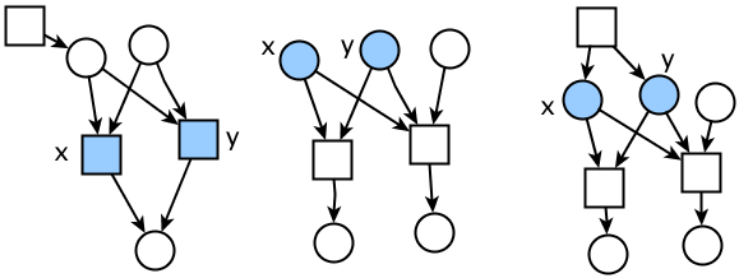
\includegraphics[width=1\linewidth]{img/reti_non_semplici.png}
        \caption{Reti non semplici}
        \label{fig:reti_non_semplici}
    \end{marginfigure}
\end{defn}

\begin{defn}
    Una rete è \textbf{pura} sse:
    \[
        \forall e \in E, \preCond{e} \cap \postCond{e} = \emptyset
    \]
    \begin{marginfigure}[-1cm]
        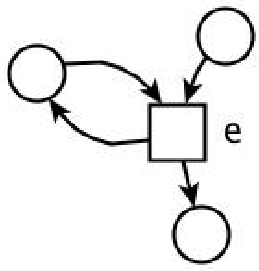
\includegraphics[width=0.4\linewidth]{img/rete_non_pura.png}
        \caption{Rete non pura.}
        \label{fig:rete_non_pura}
    \end{marginfigure}
\end{defn}

\begin{defn}
    Una transizione $t$ è \textbf{abilitata} in una rete $N$ per la
    configurazione corrente $c$, e quindi $\canFire{c}{t}{}$, sse:
    \[
        \preCond{t} \subseteq c \land \postCond{t} \cap c = \emptyset
    \]
    ovvero tutte le sue pre-condizioni sono vere, mentre tutte le sue
    post-condizioni sono false.\\
    La configurazione del sistema dopo aver eseguito $t$, indicata con $c'$,
    sarà:
    \[
        c' = \bra{c \setminus \preCond{t}} \cup \postCond{t}
    \]
    Se una transizione può essere eseguita a partire dalla configurazione $c$,
    e a seguito della transizione si raggiunge la configurazione $c'$, allora
    si scrive $\canFire{c}{t}{c'}$.
\end{defn}

\begin{defn}
    Un \textbf{passo} è un sottoinsieme di transizioni $U \subseteq T$
    indipendenti tra loro, ovvero che non condividono alcuno stato locale.
    \[
        \forall t_1, t_2 \in U, t_1 \neq t_2 \rightarrow
        (\preCond{t_1} \cup \postCond{t_1}) \cap
        (\preCond{t_2} \cup \postCond{t_2}) = \emptyset
    \]
\end{defn}

\begin{defn}
    Un \textbf{passo abilitato} per la configurazione corrente $c$ è un passo
    $U \subseteq T$ per cui:
    \[
        \forall t \in U, \canFire{c}{t}{}
    \]
    ovvero tutte le transizioni che compongono il passo sono abilitate
    per la configurazione attuale.
    Di conseguenza, tutte le precondizioni delle transizioni che compongono
    il passo devono essere verificate, mentre tutte le postcondizioni devono
    essere false.

    Le transizioni di un passo abilitato possono essere eseguite in maniera
    concorrente, ovvero possono essere eseguite contemporaneamente,
    o sequenzialmente in qualsiasi ordine.
\end{defn}

\begin{defn}
    DIAMOND PROPERTY DA FINIRE.
\end{defn}

\subsection*{Grafo dei casi e grafo dei casi sequenziale}
\begin{defn}
    L'\textbf{insieme delle configurazioni raggiungibili}
    $C_{\Sigma} \subseteq 2^{B}$, detto anche spazio degli stati,
    di un sistema elementare $\Sigma = (P, T, F, c_{\tn{start}})$
    è definito come:
    \begin{itemize}
        \item $c_{\tn{start}} \in C_{\Sigma}$
        \item $\bra{c \in C_{\Sigma} \land \exists U \subseteq T :
        \canFire{c}{U}{c'}} \rightarrow c' \in C_{\Sigma}$
    \end{itemize}
    ovvero è l'insieme di tutte le possibili configurazioni che si possono
    raggiungere all'interno del sistema elementare durante l'esecuzione.
\end{defn}

\begin{defn}
    L'\textbf{insieme dei passi} $U_{\Sigma} \subseteq 2^{T}$ di un sistema
    elementare $\Sigma$ è definito come:
    \[
        U_{\Sigma} = \cbra{U \subseteq E \, | \,
        \exists c_1, c_2 \in C_{\Sigma} : \canFire{c_1}{U}{c_2}}
    \]
    ovvero è l'insieme di tutti i possibili passi abiltati del sistema elementare.
\end{defn}

Il comportamento di un sistema elementare
può essere descritto completamente con un grafo dei casi, in cui ogni nodo
rappresenta una delle possibili configurazioni raggiungibili della rete
e ogni arco $(c_i, U, c_j)$ rappresenta l'esecuzione
$\canFire{c_i}{U}{c_j}$ di un passo abilitato $U$ per $c_i$.
Essendo gli archi etichettati con passi abilitati del sistema, il grafo
dei casi $CG_{\Sigma}$ descrive la \textbf{step semantics} del sistema
considerato.

\begin{defn}
    Il \textbf{grafo dei casi} $CG_{\Sigma}$ di un sistema elementare $\Sigma$ è
    formalmente definito come la quadrupla
    $(C_{\Sigma}, U_{\Sigma}, A, c_{\tn{start}})$ dove:
    \begin{itemize}
        \item $C_{\Sigma}$, l'insieme dei casi raggiungibili, è l'insieme
        dei nodi.
        \item $U_{\Sigma}$, l'insieme dei passi, sono le possibili etichette
        degli archi.
        \item $A = \cbra{(c, U, c') \, | \, c, c' \in C_{\Sigma} \land
        U \in U_{\Sigma} \land \canFire{c}{U}{c'}}$
        è l'insieme degli archi
        \footnote{Ogni arco è quindi etichettato con un \textit{passo},
        ovvero con un insieme di eventi del sistema $\Sigma$.}.
        \item $c_{\tn{start}}$ è la configurazione di partenza.
    \end{itemize}
\end{defn}

\begin{property}
    Il grafo dei casi gode della \textbf{diamond property}.\\
    Se un grafo dei casi $CG_{\Sigma}$ per un sistema elementare
    $\Sigma = (C_{\Sigma}, U_{\Sigma}, A, c_{\tn{start}})$ presenta gli archi
    $(c_1, U_1, c_2)$, $(c_2, U_2, c_3)$ e $(c_1, U_2, c_4)$, con
    $c_1, c_2, c_3, c_4 \in C_{\Sigma} \land U_1, U_2 \in U_{\Sigma} \land
    U_1 \cap U_2 = \emptyset$,\\
    allora sicuramente il sistema $\Sigma$ ammetterà i passi
    $(c_4, U_1, c_3)$ e $(c_1, U_1 \cup U_2, c_3)$.
    \begin{marginfigure}[1cm]
        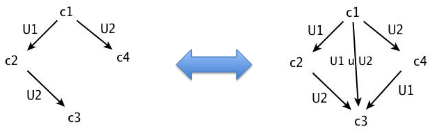
\includegraphics[width=1.05\linewidth]{img/diamond_property.png}
        \caption{Diamond property.}
        \label{fig:diamond_property}
    \end{marginfigure}
\end{property}

Gli archi del grafo dei casi sono etichettati
con \textit{sottoinsiemi} di eventi concorrenti e, per questo, la
semantica di un grafo dei casi viene detta step semantic.
In alcuni casi, però, potrebbe essere utile analizzare le possibili
sequenze di transizioni che possono essere compiute dal sistema elementare,
e queste informazioni non potrebbero essere facilmente ottenute dal grafo
dei casi.
Si può quindi definire un grafo dei caso sequenziale, in cui ogni arco è etichettato
con una singola transizione del sistema elementare e non si esprime alcuna
informazione su quali eventi possono essere eseguiti in maniera concorrente.
La semantica descritta dal grafo dei casi sequenziale prende il nome
di semantica a \textbf{interleaving}, e altro non è
che una simulazione sequenziale non deterministica del sistema.

\begin{defn}
    Il \textbf{grafo dei casi sequenziale} $SCG_{\Sigma}$ di una rete
    di Petri $\Sigma$ è una quadrapla $(C_{\Sigma}, T, A, c_{\tn{start}})$
    dove:
    \begin{itemize}
        \item $C_{\Sigma}$, l'insieme dei casi raggiungibili, è l'insieme dei
        nodi.
        \item $T$, l'insieme delle transizioni, è l'alfabeto del grafo con cui
        verranno etichettati gli archi.
        \item $A = \cbra{(c, t, c') \, | \, c, c' \in C_{\Sigma} \land
        t \in T \land \canFire{c}{t}{c'}}$
        è l'insieme degli archi.
        \item $c_{\tn{start}}$ è la configurazione di partenza.
    \end{itemize}
\end{defn}

\begin{marginfigure}
    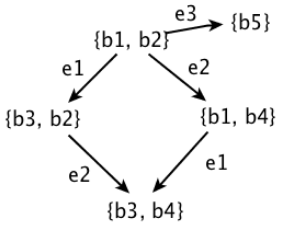
\includegraphics[width=0.60\linewidth]{img/grafo_casi_sequenziale.png}
    \caption{Grafo dei casi sequenziale.}
    \label{fig:sequential_case_graph}
\end{marginfigure}

Il grafo dei casi sequenziale è un \textit{sistema a transizioni
etichettato} che modella il sistema concorrente preso in analisi,
e può quindi essere usato per verificare alcune proprietà del sistema
concorrente che si sta analizzando, come la presenza di deadlock.
Data una rete di Petri, però, trovare l'insieme delle configurazioni
raggiungibili, necessario per costruire il grafo dei casi sequenziale,
può essere complesso e portare a un'esplosione combinatoria: per questo motivo,
le reti di Petri vengono usate per verificare solo alcune proprietà facilmente
determinabili, mentre negli altri casi si preferiscono altri modelli
formali, come le logiche temporali.

\begin{property}
    Il grafo dei casi $CG_{\Sigma}$ e il grafo dei casi sequenziale
    $SCG_{\Sigma}$ dello stesso sistema elementare $\Sigma$ sono
    \textbf{sintatticamente equivalenti}, ovvero è possibile ottenere uno a
    partire dall'altro usando solo procedimenti di modifica sintattica.
    In particolare, un grafo dei casi sequenziale può essere costruito
    da un grafo dei casi semplicemente rimuovendo tutti gli archi
    etichettati con un passo di cardinalità strettamente maggiore di 1.
    Viceversa, un grafo dei casi può essere costruito a partire da un
    grafo dei casi sequenziale usando la diamond property.
\end{property}

\begin{rem}
    Dato un sistema elementare, trovare un sistema di transizioni etichettato
    che modella il suo comportamento è molto semplice: basta infatti costruire
    il grafo dei casi sequenziale.
    Trovare invece un sistema elementare il cui grafo dei casi sequenziale
    è isomorfo a un dato sistema a transizioni etichettato risulta più
    complicato. Il problema viene comunque risolto usando la teoria delle regioni.
\end{rem}

\section{Situazioni particolari}
\subsection*{Contatto}
\begin{defn}
    Siano $\Sigma = (P, T, F, c_{\tn{start}})$ un sistema elementare, $t \in T$
    una transizione e $c \in C_{\Sigma}$ una possibile configurazione di $\Sigma$,
    $(t, c)$ è un \textbf{contatto} sse:
    \[
        \preCond{t} \subseteq c \land \postCond{t} \cap c \neq \emptyset
    \]
    ovvero tutte le pre-condizioni di $t$ sono vere, ma almeno una
    post-condizione di $t$ è vera.\\
    Una transizione che si trova in uno stato di contatto non è abilitata.
\end{defn}

\begin{rem}
    Una transizione senza precondizioni è sicuramente un contatto: viene
    infatti eseguita subito, in quanto l'insieme vuoto delle precondizioni
    è sempre vero, e quindi le post-condizioni diventano vere.
    Ma poi la transizione, non
    avendo pre-condizioni, avrà sicuramente le pre-condizioni vere e tutte
    le post-condizioni vere. Di conseguenza si ha un contatto.
\end{rem}

\begin{defn}
    Un sistema elementare $\Sigma = (P, T, F, c_{\tn{start}})$ è un
    \textbf{sistema senza contatti} sse:
    \[
        \forall t \in T, \forall c \in C_{\Sigma} \quad
        \preCond{t} \subseteq c \rightarrow \postCond{t} \cap c = \emptyset
    \]
    ovvero, qualunque sia la configurazione del sistema, se le pre-condizioni
    di una transizione sono vere, allora sicuramente tutte le sue post-condizioni
    sono false, e la transizione è abilitata \footnote{In un sistema elementare
    senza contatti, per stabilire se una transizione è abilitata non è necessario
    effettuare alcun controllo sulle post-condizioni: se le pre-condizioni
    sono vere, infatti, le post-condizioni saranno sicuramente false.}.
    Un sistema senza contatti ha un importante vantaggio: per stabilire
    se una transizione è abilitato non è necessario analizzare le sue
    post-condizione, ma serve solo verificare se tutte le pre-condizioni
    sono vere.
\end{defn}

\subsection*{Rimozione dei contatti}
Ogni sistema elementare $\Sigma$ con contatti può essere trasformato in un
sistema elementare $\Sigma'$ senza contatti e con grafo dei casi isomorfo.
\begin{defn}
    Due posti $p, q \in P$ sono \textbf{complementari} sse:
    \[
        \preCond{p} = \postCond{q} \land \preCond{q} = \postCond{p}
        \land \bra{p \in c_{\tn{start}} \oplus q \in c_{\tn{start}}}
    \]
    ovvero le post-condizioni di uno sono le pre-condizioni dell'altro
    e viceversa, ed esattamente uno dei posti appartiene alla configurazione
    iniziale del sistema elementare.
\end{defn}

\begin{marginfigure}
    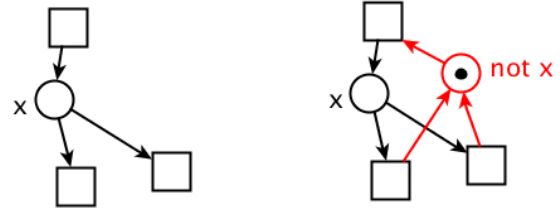
\includegraphics[width=0.85\linewidth]{img/contatto_complementare.png}
    \caption{Rimozione di un contatto tramite l'aggiunta dello stato complementare.}
    \label{fig:sistema_con_contatti}
\end{marginfigure}

Per rimuovere tutti i contatti da un sistema elementare devono essere
aggiunti posti complementari ad ogni posto del sistema elementare,
se non sono ancora presenti, e si deve garantire che esattamente
un posto tra posto e posto complementare appartenga alla configurazione
iniziale.
L'insieme delle transizioni del sistema elementare rimane invece invariato,
ovvero non vengono aggiunte o rimosse transizioni dal sistema.

\begin{figure}
    \centering
    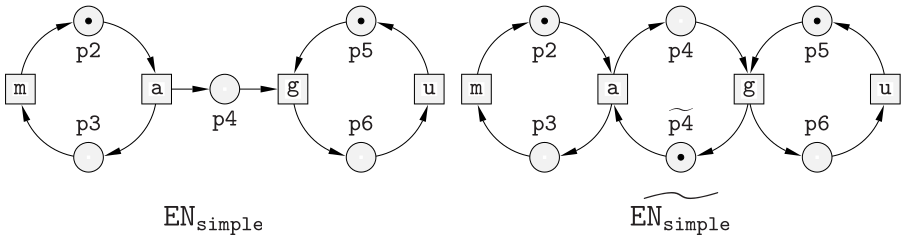
\includegraphics[width=\linewidth]{img/sistema_senza_contatti.png}
    \caption{Rimozione dei contatti da un sistema con contatti.}
    \label{fig:sistema_senza_contatti}
\end{figure}

\subsection*{Conflitto}
\begin{defn}
    Siano $\Sigma = (P, T, F, c_{\tn{start}})$ un sistema elementare,
    $t_1, t_2 \in T$ due transizioni e $c \in C_{\Sigma}$ una possibile
    configurazione di $\Sigma$, $t_1$ ed $t_2$ sono in \textbf{conflitto}
    in $c$ sse:
    \[
        \canFire{c}{t_1}{} \land \canFire{c}{t_2}{} \land
        \lnot \canFire{c}{\cbra{t_1, t_2}}{}
    \]
    ovvero entrambe le transizioni sono abilitate, ma il verificarsi di una
    rende l'altra non abilitata. Di conseguenza, le due transizioni non
    possono essere eseguite in maniera concorrente. Non sapendo quale
    delle due transizioni verrà effettivamente eseguite, un conflitto esprime
    non determinismo.

    \begin{marginfigure}
        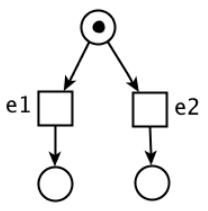
\includegraphics[width=0.75\linewidth]{img/conflitto_avanti.png}
        \caption{Conflitto in avanti.}
        \label{fig:conflitto_avanti}
    \end{marginfigure}

    \begin{marginfigure}
        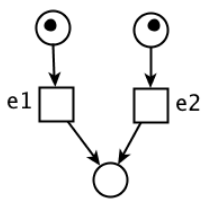
\includegraphics[width=0.75\linewidth]{img/conflitto_indietro.png}
        \caption{Conflitto all'indietro.}
        \label{fig:conflitto_indietro}
    \end{marginfigure}

    Esistono due tipi di conflitti:
    \begin{itemize}
        \item in avanti: due transizioni abilitate condividono almeno una
        pre-condizione.
        Il verificarsi di una transizione rende falsa la pre-condizione in comune,
        disabilitando l'altra transizione;
        \item all'indietro: due transizioni abilitate condividono almeno una
        post-condizione. Il verificarsi di una transizione rende vera la
        post-condizione in comune, disabilitando l'altra transizione.
    \end{itemize}

    \begin{rem}
        Un conflitto tra transizioni rappresenta una competizione
        per l'utilizzo di risorse condivise.
    \end{rem}
\end{defn}

\subsection*{Confusione}
La confusione si presenta in un sistema con conflitti in cui la struttura non
permette di stabilire se, nel passaggio da una configurazione $c$ a una
configurazione $c'$, è stato risolto un conflitto.

\begin{figure}
    \centering
    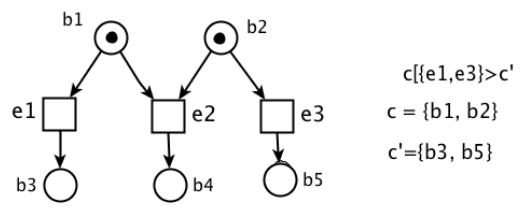
\includegraphics[width=0.5\linewidth]{img/confusione.png}
    \label{fig:confusione}
\end{figure}
In questo sistema non è possibile stabilire se, passando da $c$ a $c'$, sia
stato risolto un conflitto tra $e_1$ ed $e_2$ o tra $e_2$ ed $e_3$.

Un altro esempio di confusione si verifica nella mutua esclusione.

\subsection*{Sequenza}
Siano $\Sigma = (P, T, F, c_{\tn{start}})$ un sistema elementare,
$t_1, t_2 \in E$ due transizioni e $c \in C_{\Sigma}$ una possibile configurazione
di $\Sigma$, $t_1$ ed $t_2$ sono in \textbf{sequenza} in $c$ sse:
\[
    \canFire{c}{t_1}{} \land \lnot \canFire{c}{t_2}{} \land
    \canFire{\canFire{c}{t_1}{c'}}{t_2}
\]
ovvero $t_2$ può essere eseguito sse prima viene eseguito $t_1$.
C'è quindi una dipendenza causale tra le transizioni $t_1$ ed $t_2$.

\begin{figure}
    \centering
    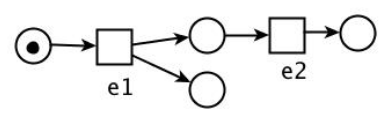
\includegraphics[width=0.5\linewidth]{img/sequenza.png}
    \caption{Due eventi in sequenza.}
    \label{fig:eventi_sequenza}
\end{figure}

\subsection*{Concorrenza}
Siano $\Sigma = (P, T, F, c_{\tn{start}})$ un sistema elementare,
$t_1, t_2 \in E$ due transizioni e $c \in C_{\Sigma}$ una possibile configurazione
di $\Sigma$, $t_1$ ed $t_2$ sono \textbf{concorrenti} in $c$ sse:
\[
    \canFire{c}{\cbra{t_1, t_2}}{}
\]
ovvero $\cbra{t_1, t_2}$ è un passo abilitato. Questo significa che le due
transizioni $t_1$ ed $t_2$ sono indipendenti ed entrambe abilitate in $c$:
esse possono essere eseguite contemporaneamente o sequenzialmente in qualsiasi
ordine.

\begin{figure}
    \centering
    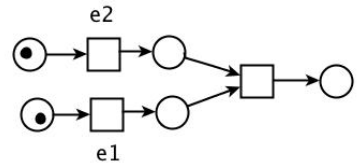
\includegraphics[width=0.5\linewidth]{img/eventi_concorrenti.png}
    \caption{Due transizioni concorrenti.}
    \label{fig:eventi_concorrenti}
\end{figure}

\begin{thm}
    Si considerino solo le relazioni di sequenza, conflitto e concorrenza tra
    transizioni.
    Se una transizione si trova in una delle tre relazioni ad una certa configurazione,
    allora sicuramente non si troverà mai nelle altre due relazioni, qualsiasi
    sia la configurazione in cui si trovi la rete.
\end{thm}

\section{Equivalenza semantica tra sistemi elementari}
Il primo approccio che si può utilizzare per verificare l'equivalenza
semantica di due sistemi elementari è verificare l'isomorfismo
dei due sistemi elementari stessi. L'isomorfismo è, però, una relazione
di equivalenza troppo restrittiva per l'equivalenza semantica: di fatto,
un certo tipo di comportamento sarebbe descritto solo da un tipo di rete.\\
Si può quindi provare a verificare l'isomorfismo dei grafi dei casi
sequenziale: risulta, infatti, una relazione di equivalenza meno
restrittiva e permette di considerare semanticamente equivalenti anche
sistemi elementari diversi, a patto che abbiano lo stesso caso dei grafi
sequenziale. Un esempio di sistemi elementari diversi ma con lo stesso
caso dei grafi sequenziale è quello dei sistemi senza contatto: un sistema
con contatti e il relativo sistema senza contatti, infatti, hanno
grafo dei casi isomorfo.\\
Anche l'isomorfismo dei grafi dei casi sequenziale può risultare, però,
troppo restrittivo per analizzare l'equivalenza semantica di due sistemi
elementari. Si può notare, però, che i grafi dei casi sono sistemi
di transizione etichettati, e di conseguenza è possibile definire la nozione
di bisimulazione, allo stesso modo del CCS. Allo stesso modo del CCS,
inoltre, la bisimulazione può essere verificata usando il gioco
dell'attaccante-difensore.


\section{Processi non sequenziali e processi ramificati FINIRE}
DA SISTEMARE L'ITALIANO
Grafo dei casi e grafo dei casi sequenziale esprimono rispettivamente
la step semantic e la semantica a interleaving del sistema elementare
a cui fanno riferimento.
Entrambe le semantiche, però, esprimono il comportamento del sistema
elementare come una simulazione sequenziale non deterministica: nel primo caso,
le sequenze sono composte da passi abilitati, mentre nel secondo sono composte
da transizioni. Non è quindi possibile ottenere informazioni riguardo
all'indipendeza e la causalità tra le transizioni, e anche riguardo la
concorrenza nel solo grafo dei casi sequenziale.
Le reti di Petri offrono però un metodo formale per descrivere il comportamento
della rete evidenziando causalità e concorrenza tra transizioni, in modo
che queste informazioni siano facilmente ottenibili, e questo prende
il nome di semantica a processi.
Prima di poter spiegare cosa sono i processi non sequenziali e i processi
ramificati, è necessario introdurre alcune nozioni.

\subsection*{Relazioni sugli elementi di una rete}
\begin{defn}
    La relazione d'ordine parziale largo \footnote{Una relazione d'ordine largo
    è una relazione riflessiva, antisimmetrica e transitiva.}
    $\le \, \subseteq (B \cup E) \times (B \cup E)$ specifica se un elemento
    è causa di un altro elemento, ed è definita come:
    \[
        \forall x, y \in B \cup E, \quad (x, y) \in \, \le \quad
        \tn{ sse } \quad x F^*y
    \]
    ovvero è possibile raggiungere $y$ a partire da $x$ usando un numero
    limitato di transizioni. Se $(x,y) \in \, \le$, allora $x$ causa $y$.
    Si può notare che, in questa relazione, un elemento $x$ causa sè stesso.
\end{defn}

\begin{defn}
    La relazione d'ordine parziale stretto \footnote{Una relazione d'ordine
    stretto è una relazione irriflessiva, asimmetrica e transitiva.}
    $< \, \subseteq (B \cup E) \times (B \cup E)$ specifica se un elemento
    è causa di un altro elemento diverso da sè stesso, ed è definita come:
    \[
        \forall x, y \in B \cup E, \quad (x, y) \in \, < \quad \tn{ sse } \quad
        x F^*y \land x \neq y
    \]
\end{defn}

\begin{rem}
    $<$ è facilmente ottenibile da $\le$ rimuovendo tutte le coppie della forma
    $(x,x), \forall x \in B \cup E$.
\end{rem}

\begin{defn}
    Sia $N$ una rete di Petri, la \textbf{relazione di conflitto}
    $\# \subseteq P \cup T$ specifica quali coppie di elementi della rete $N$
    sono causalmente dipendenti da un conflitto in avanti, ed è definita come:
    \[
        x \# y \quad \tn{ sse } \quad \exists e_1, e_2 \in E,
        (e_1 \neq e_2 \land e_1 \le x \land e_2 \le y) :
        \preCond{e_1} \cap \preCond{e_2} \neq \emptyset
    \]
\end{defn}

\begin{rem}
    La relazione di conflitto $\#$ è simmetrica ma non transitiva.
\end{rem}

\begin{defn}
    La relazione $\tn{li} \subseteq (B \cup E) \times (B \cup E)$ specifica
    quali elementi della rete sono causalmente dipendenti, ed è definita come:
    \[
        \forall x, y \in B \cup E, \quad (x, y) \in \tn{ li} \quad
        \tn{ sse } \quad (x,y) \in \, \le \lor \, (y,x) \in \, \le
    \]
\end{defn}

\begin{defn}
    La relazione $\tn{co} \subseteq (B \cup E) \times (B \cup E)$ specifica
    quali elementi della rete sono causalmente indipendenti, ed è definita come:
    \[
        \forall x, y \in B \cup E, \quad (x, y) \in \tn{ co} \quad \tn{ sse } \quad
        (x,y) \notin \, < \land \, (y,x) \notin \, < \land \, (x,y) \notin \#
    \]
\end{defn}

\begin{rem}
    \begin{align*}
        (x,y) \in \tn{ li } &\longleftrightarrow (y,x) \in \tn{ li}\\
        (x,y) \in \tn{ co } &\longleftrightarrow (y,x) \in \tn{ co}
    \end{align*}
\end{rem}
\begin{rem}
    $\tn{li}$ e $\tn{co}$ sono relazioni riflessive, simmetriche ma non
    transitive.
\end{rem}

\subsection*{Tagli e linee}
\begin{defn}
    Un \textbf{coset} $C \subseteq P \cup T$ è un insieme di elementi
    della rete di Petri tale che:
    \[
        \forall x, y \in C, x \tn{ co } y
    \]
    ovvero gli elementi di un coset sono tutti causalmente indipendenti tra
    loro.
\end{defn}

\begin{rem}
    In un coset, la relazione $\tn{co}$ è transitiva.
\end{rem}

\begin{defn}
    Un \textbf{taglio} $C \subseteq P \cup T$ è un coset massimale, ovvero:
    \[
        C \tn{ è un coset } \, \land \, \forall x \in (B \cup E) \setminus C, \,
        \exists c \in C : x \tn{ li } c
    \]
    ovvero ogni altro elemento che non appartiene a $C$ è causalmente
    dipendente da almeno un elemento di $C$, o viceversa.
\end{defn}

\begin{defn}
    Un taglio $C$ è un \textbf{P-taglio} sse $C \subseteq P$, ovvero è formato
    da soli stati locali.
\end{defn}

\begin{rem}
    Un P-taglio corrisponde a uno dei possibili casi raggiungibili della rete.
    Di conseguenza, tutti i possibili P-tagli definiscono tutti i possibili
    casi raggiungibili della rete.
\end{rem}

\begin{defn}
    Un taglio $C$ è un \textbf{T-taglio} sse $C \subseteq T$, ovvero è formato
    da soli eventi.
\end{defn}

\begin{rem}
    Tutti gli eventi all'interno di un T-taglio possono essere eseguiti in
    maniera concorrente. Essendo un T-taglio l'insieme di cardinalità massima
    $n$ che contiene solo eventi indipendenti tra loro, il sistema necessita
    di $n$ processori per l'esecuzione in minor tempo possibile degli $n$
    eventi.\\
    Il numero di processori per una rete (da cui si deriva la rete di
    occorrenze), è pari alla cardinalità massima tra le cardinalità degli
    T-tagli di tutti i processi non sequenziale che è possibile definire.
\end{rem}

\begin{defn}
    Un \textbf{liset} $L \subseteq P \cup T$ è un insieme di elementi della
    rete di Petri tale che:
    \[
        \forall x, y \in L, x \tn{ li } y
    \]
    ovvero gli elementi di un liset sono tutti causalmente dipendenti tra loro.
\end{defn}

\begin{rem}
    In un liset, la relazione $\tn{li}$ è transitiva.
\end{rem}

\begin{defn}
    Una \textbf{linea} $L \subseteq P \cup T$ è un liset massimale, ovvero:
    \[
        L \tn{ è un coset } \, \land \, \forall x \in (B \cup E) \setminus L, \,
        \exists l \in L : x \tn{ co } l
    \]
    ovvero ogni altro elemento che non appartiene a $L$ è causalmente
    indipendente da almeno un elemento di $C$, o viceversa.
\end{defn}

\begin{defn}
    Una rete è \textbf{\textit{k}-densa} se ogni linea si interseca una singola
    volta con ogni altro taglio e, viceversa, ogni taglio si interseca una
    singola volta con ogni altra linea.
\end{defn}

Un taglio e una linea si intersecano esattamente in un punto perchè se si
incontrassero in più punti, allora tutti i punti di intersezione
rappresenterebbero elementi che sono contemporaneamente casualmente
dipendenti (li) e casualmente indipendenti (co), violando quindi i tagli
e le linee definite.

\begin{rem}
    Una rete finita è sicuramente $k$-densa.
\end{rem}

\subsection*{Processo ramificato}
\begin{defn}
    Una \textbf{rete di occorrenze} è una rete $(P, T, F)$ tale che:
    \begin{itemize}
        \item $\forall p \in P, |\preCond{p}| = 1$, ovvero non sono
        accettati conflitti all'indietro. Sono invece accettati
        i conflitti in avanti.
        \item $\forall x, y \in P \cup T, (x,y) \in F^+ \rightarrow
        (y,x) \notin F^+$, ovvero non sono presenti cicli.
        \item $\forall e \in T$, l'insieme $\cbra{x \in P \cup T : x F^*e}$,
        ovvero il passato di ogni evento, ha cardinalità finita.
        \item la relazione di conflitto $\#$ è irriflessiva \footnote{E di
        conseguenza antisimmetrica.}, ovvero un unico elemento non dipende
        causalmente da due eventi in conflitto in avanti.
    \end{itemize}
\end{defn}

Su una rete di occorrenze è possibile definire le funzioni
\begin{align*}
    \tn{past}: P \cup T &\rightarrow \mathcal{P}(P \cup T)\\
    \tn{future}: P \cup T &\rightarrow \mathcal{P}(P \cup T)
\end{align*}

$\tn{past}$ restituisce tutti gli elementi della rete che causano $x$, mentre
$\tn{future}$ restituisce tutti gli elementi che sono causati da $x$.\\
Per definizione di rete di occorrenze, $\tn{past}(x)$ è sicuramente un insieme
di cardinalità finita, mentre $\tn{past}(x)$ può avere cardinalità infinita
numerabile.

\begin{rem}
    Tutti gli elementi della rete che non appartengono nè a $\tn{past}(x)$ nè
    a $\tn{future}(x)$ possono essere eseguiti in maniera concorrente rispetto
    a $x$.
\end{rem}

\begin{defn}
    Un \textbf{processo ramificato} di un sistema elementare
    $\Sigma_1 = (P_1, T_1, F_1, c_1)$ senza contatti e finito (e quindi $k$-densa),
    è una coppia $(\Sigma_2, \phi), \Sigma_2 = (P_2, T_2, F_2, c_2)$ tale che:
    \begin{itemize}
        \item $\Sigma_2$ è una rete di occorrenze;
        \item $\phi: P_2 \cup T_2 \rightarrow P_1 \cup T_1$ è una funzione
        tale che:
        \begin{itemize}
            \item $\phi(P_2) \subseteq P_1 \land \phi(T_2) \subseteq T_1$,
            ovvero gli elementi della rete $\Sigma_2$ del processo ramificato
            rappresentano elementi del sistema elementare $\Sigma$.
            \item $\forall e_1, e_2 \in T_2, \, (\preCond{e_1} = \preCond{e_2}
            \land \phi(e_1) = \phi(e_2)) \implies e_1 = e_2$, ovvero
            se due transizioni della rete $\Sigma_2$ associata al processo
            ramificato hanno le stesse pre-condizioni e rappresentano lo
            stesso elemento del sistema elementare $\Sigma_1$, allora sono
            lo stesso elemento nella rete $\Sigma_2$ del processo ramificato
            SISTEMARE ITALIANO.
            \item MANCA 1
            \item MANCA 2
        \end{itemize}
    \end{itemize}
\end{defn}

\begin{rem}
    La configurazione iniziale di un processo ramificato comprende tutti i
    posti della sua rete che non presentano archi in ingresso, e rappresenta
    la configurazione raggiugibile del sistema elementare che si sta trattando
    da cui inizia l'esecuzione descritta dal processo ramificato.
\end{rem}

\begin{rem}
    Un processo ramificato contiene una o più run della rete di Petri da cui
    è stato costruito.
\end{rem}

\subsection*{Processo non sequenziale}
Una rete causale è un tipo particolare di rete di occorrenze, che non presenta
alcun conflitto.\\
\begin{defn}
    Una \textbf{rete causale} è una rete $(P, T, F)$ tale che:
    \footnote[][-1cm]{L'ulteriore condizione presente nelle reti di occorrenza,
    ovvero che la relazione di conflitto sia irriflessiva, collassa nella prima
    condizione per le reti clausali: non avendo alcun conflitto, per la rete
    clausale vale $\# = \emptyset$.}:
    \begin{itemize}
        \item $\forall p \in P, \lvert \preCond{p} \rvert \le 1 \land \lvert \postCond{p} \rvert \le 1$,
        ovvero non sono presenti conflitti \footnote[][1cm]{In un conflitto in
        avanti, lo stato pre-condizione ha due post-eventi. In un conflitto
        all'indietro, lo stato post-condizione ha due pre-eventi. Di conseguenza,
        imporre un numero di pre-eventi e post-eventi minore o uguale a uno implica
        l'assenza di conflitti.};
        \item $\forall x, y \in P \cup T, \quad (x, y) \in T^+ \rightarrow (y, x) \notin T^+$,
        ovvero non sono presenti cicli;
        \item $\forall t \in T$, la cardinalità dell'insieme $\cbra{x \in P \cup T | x \, T^* e}$
        è finita, ovvero i predecessori di un qualsiasi evento sono in numero
        finito.
    \end{itemize}
\end{defn}

\begin{rem}
    Una rete causale ammette elementi isolati, ovvero elementi senza archi
    in ingresso e archi in uscita.
\end{rem}

\begin{defn}
    Un \textbf{processo non sequenziale} di un sistema elementare
    $\Sigma_1 = (P_1, T_1, F_1, c_1)$ senza contatti e finito (e quindi $k$-densa),
    è una coppia $(\Sigma_2, \phi), \Sigma_2 = (P_2, T_2, F_2, c_2)$ tale che:
    \begin{itemize}
        \item $\Sigma_2$ è una rete causale;
        \item $\phi: P_2 \cup T_2 \rightarrow P_1 \cup T_1$ è una funzione tale che:
        \begin{itemize}
            \item FINIRE
        \end{itemize}
    \end{itemize}
\end{defn}

\begin{rem}
    Un processo non sequenziale rappresenta una sola delle possibili
    esecuzioni del sistema concorrente.
\end{rem}

\subsection*{Prefisso e unfolding}
\begin{defn}
    Sia $\Sigma = (S, T , F , c_in)$ un sistema elementare finito e senza contatti
    e siano $\Pi_1 = (N_1, \phi_1)$, $\Pi_2 = (N_2, \phi_2)$ due suoi processi
    ramificati.
    $\Pi_1$ è un prefisso di $\Pi_2$ sse:
    \begin{itemize}
        \item $N_1$ è una sottorete di $N_2$
        \item $\phi_2|N_1 = \phi_1$, ovvero $\phi_2$ ”ristretto” a $N_1$ è
        uguale a $\phi_1$.
    \end{itemize}
\end{defn}

\begin{defn}
    L'\textbf{unfolding} di una rete elementare $\Sigma$ è il processo ramificato
    massimale, ovvero il processo ramificato che include tutte le possibili
    run di $\Sigma$.
\end{defn}

\begin{rem}
    Ogni processo ramificato (compresi i processi non sequenziali, in quanto
    sono casi particolari di processi ramificati con una singola run) è un
    prefisso dell'unfolding.
\end{rem}

è possibile anche cercare di individuare un prefisso finito dell'unfolding
che permetta di derivare tutte le possibili informazioni riguardo il comportamento
del sistema elementare. Questo prefisso prende il nome di prefisso completo.


\section{Estensioni}
Fino ad ora sono state considerate solo le reti elementari, ovvero
reti di Petri che tollerano al massimo un token per stato e che
prevedono che ogni transizione sottragga un token da ogni precondizione, e
ne aggiunga uno a ogni postcondizione.

\upperAccE possibile, però, definire reti di Petri in cui ogni stato
può contenere più token, e in cui ogni arco assume un peso, ovvero elabora
un numero di token, diverso da 1 \footnote{In entrambi i casi,
la capacità del posto e il peso dell'arco vengono indicati graficamente
affiancando il numero all'elemento considerato.}. D'ora in poi, queste
reti verranno definite \textit{reti ad alto livello}.

Queste reti di Petri non hanno però una maggiore capacità espressiva
dei sistemi elementari: si può dimostrare, infatti, che
ogni sistema elementare può essere simulato usando una rete ad alto livello
e, viceversa, una rete ad alto livello può essere simulata con
un sistema elementare.
Le reti ad alto livello presentano, però, un vantaggio rispetto ai sistemi
elementari: esse risultano, infatti, più compatte rispetto ai sistemi
elementari e, di conseguenza, più facilmente trattabili.
Proprietà come la boundness, la safeness, la terminazione,
la presenza di deadlock e la liveness possono, infatti, essere verificate
algoritmicamente, in un tempo accettabile, su reti di questo tipo.

Un'altra possibile estensione ai sistemi elementari riguarda la tipologia
dei token: in un sistema elementare, e più in generale in una rete di
Petri, tutti i token rappresentano lo stesso tipo di dato astratto, e
ogni transizione può trattare qualsiasi token che circola nella rete.
\upperAccE possibile, però, definire reti di Petri in cui i token
possono assumere colori differenti, e in cui le transizioni possono
trattare solo i token dei colori su cui sono state definite.
Questo tipo di rete prende il nome di \textit{rete colorata}, e permette
di rappresentare, tramite i diversi colori che i token possono assumere,
diversi tipi di dati astratti che circolano nella rete.

\subsection*{Rappresentazione algebrica delle reti di Petri}
Una rete ad alto livello in cui ogni stato ha capacità infinita
e non sono presenti cappi è rappresentabile usando una matrice di incidenza,
in cui le righe corrispondono ai posti della rete, mentre le colonne
rappresentano le transizioni della rete.
Una generica cella della matrice $(i, j)$ contiene il peso
dell'arco che collega il posto di indice $i$ alla transizione di indice $j$ o,
viceversa, l'arco che collega la transizione di indice $j$ al posto
di indice $i$. Se un arco non è presente nella rete, allora la relativa
cella nella matrice di incidenza rimane vuota.\\
Le configurazioni della rete, invece, vengono specificate
come colonne aggiuntive, che si affiancano alle colonne delle transizioni:
una colonna rappresentante una configurazione conterrà, nella sua $i$-esima
riga, il numero di token contenuti all'interno dello stato di indice $i$.

La matrice di incidenza è utile per descrivere algebricamente
le transizioni che avvengono nella rete.
Sia infatti $M_i$ la configurazione corrente della rete, rappresentata
da un'apposita colonna, allora la configurazione della rete raggiunta
a seguito della transizione abilitata $t$ può essere facilmente trovata
sommando la colonna associata a $M_i$ e la colonna associata a $t$.\\
Si può affermare, quindi, che una configurazione $M_1$ è raggiungibile
da $M_0$ allo scattare di $t$, ovvero $M_0[t>M_1$, sse $M_0 + t = M_1$.
Questa equazione prende il nome di \textit{equazione di stato}.

\section{CAAL: un tool per le reti di Petri}
